\chapter[Génération et évaluation des explications dans la littérature]{Génération et évaluation des explications dans la littérature} \label{C1}

\boitemagique{Dans ce chapitre}{
Ce chapitre présente l'état de l'art en XAI, divisé en trois sections. La première partie reprend la typologie des explications d'IA de la littérature. La seconde porte sur la génération de ces explications, et la troisième porte sur leur évaluation.
Nous mettons en avant la multiplicité des méthodes de création des explications. En effet, il n'y a pas une méthode qui conviendrait à tous les usages, ce qui a conduit à de nombreuses propositions de la communauté XAI.
De même, il n'existe pas de consensus sur la manière d'évaluer les explications, que ce soit sur le protocole ou les métriques présentées. Nous présentons un large panel de propositions, ainsi que leurs avantages et inconvénients.
}
% Objectif de la section
Ce chapitre présente diverses méthodes de génération d'explication de la littérature, ainsi que des méthodes d'évaluation de ces explications. Cet état de l'art aborde deux problématiques de l'explicabilité de l'intelligence artificielle (XAI). La première est : comment obtenir un outil d'intelligence artificielle explicable? La seconde est: comment évaluer la méthode d'explicabilité d'un outil?

% Comment
Une explication peut être créée via des méthodes variées et peut prendre diverses formes. Pour un même outil, il est possible de chercher des explications différentes répondant à des objectifs variés. Ces besoins différents ont amené à la création d'un grand nombre de solutions dans la littérature.

\'Evaluer une explication nécessite donc de s'assurer que celle-ci est bien conçue par l'expliqueur, mais également bien perçue par le receveur.
Les méthodes d'évaluation sont tirées des explications elles-mêmes, basées sur le ressenti subjectif d'un utilisateur ou sur l'impact objectif d'une explication dans une tâche. Le choix d'une évaluation adaptée rend compte non seulement de la qualité d'une explication mais aussi de son adéquation avec les objectifs de l'outil global dans la réalisation d'une tâche.

% Plan
Nous définissons d'abord les différents types d'explications en section \ref{C1:typologie}.
Nous présentons ensuite en section \ref{C1:generation} les principales méthodes d'explication, et en section \ref{C1:evaluations} les évaluations de ces explications.


\section{Typologie des méthodes d'explication} \label{C1:typologie}

Le choix d'une méthode est notamment guidé par des contraintes techniques ou d'organisation du projet : nature du modèle à expliquer, détection de la problématique d'explicabilité avant ou après conception du modèle, etc. Cette section passe en revue quatre caractéristiques permettant de définir une méthode d'explication : la portée, la stratégie, le format, et les données d'application. La typologie est inspirée d'états de l'art fondateurs dans le domaine~\cite{Guidotti2018, Gilpin2018, Dam2018, Hohman2018, molnar2019, Beaudouin2020, Arrieta2020}.

\subsection{Portée : globale vs. locale}

La portée des explications données par une méthode peut être locale ou globale. Ces deux types d'explications n'ont pas le même objectif.
Les facteurs permettant de choisir entre une explication globale ou locale sont :
\begin{itemize}
    \item le but de l'explication,
    \item les questions auxquelles elle doit répondre,
    \item le public ciblé,
    \item le contexte de réception de l'explication.
\end{itemize}
Pour chacun de ces points, l'une ou l'autre portée sera à privilégier.

\paragraph{Globale}

Une explication globale s'applique au modèle dans son ensemble. Elle est vraie pour toute entrée, et permet de comprendre le comportement du modèle dans les cas nominaux et extraordinaires.
% \item le but de l'explication - QUOI
Son but est de donner une vision globale du modèle, pour tout résultat possible.
Elle permet de construire la confiance dans le modèle et valider la mise en place de ce dernier.

% \item les questions auxquelles elle doit répondre - POURQUOI
Les questions abordées sont :
\begin{itemize}
    \item Quels sont les points faibles de mon modèle ?
    \item Dans quels cas puis-je l'utiliser sans crainte ?
    \item Dans quels cas dois-je me méfier ?
    \item Comment a-t-il appris ?
    \item Quelles sont les données d'entraînement pertinentes ?
    \item Quel est l'intérêt/la contribution de cette sous partie de mon modèle pour la réalisation de la tâche ?
    \item comment modifier mes données d'entraînement afin de gagner en performances ?
\end{itemize}

% \item le public ciblé
Le public cible de ces explications est constitué de scientifiques des données, d'experts du domaine d'application, de décideurs et d'utilisateurs finaux.~\cite{Mitchell2019}
% \item le contexte de réception de l'explication
Les explications globales sont particulièrement adaptées pour mesurer les performances et améliorer le modèle, définir ses limites d'applications, valider la mise en production du modèle, et instaurer une phase d'appropriation pour les utilisateurs finaux.

\paragraph{Locale}
Une explication locale s'applique pour un modèle et une instance donnée. Elle permet de comprendre pourquoi pour une entrée définie, le modèle donne un résultat et non un autre.
% \item le but de l'explication - Quoi
Elle met en lumière le raisonnement du modèle dans un cas précis, voire dans un groupe d'instances plus étendu mais défini. Elle permet de construire la confiance dans le résultat, sans généraliser au reste du modèle.

Les questions auxquelles elle doit répondre sont:
\begin{itemize}
    \item Pourquoi j'obtiens ce résultat avec cette entrée ?
    \item Que changer en entrée pour changer le résultat en sortie ?
    \item Que se passe-t-il si ma donnée d'entrée change sur cette variable ?
\end{itemize}
% \item le public ciblé
Ces explications ciblent en priorité les utilisateurs finaux, ainsi que les experts du modèle.
% \item le contexte de réception de l'explication
Ce format est adapté pour une intégration aux conditions réelles d'utilisation d'un modèle. Il se concentre sur le résultat obtenu par l'utilisateur. Il est également indiqué si l'utilisateur a peu de temps pour lire l'explication.

% transition
En résumé, une explication globale demande plus de temps qu'une explication locale. Mais la première permet de faire la lumière sur tout le modèle, là où l'explication locale donne confiance dans un exemple en particulier. Ainsi, une explication globale sera plus pertinente pour un audit ou une évaluation globale du modèle. Une explication locale sera plus efficace à l'usage en conditions réelles, ou pour l'étude approfondie de cas spécifiques. Outre la portée, différentes stratégies d'explicabilité peuvent être mises en place.

\subsection{Stratégie}

On peut classer ces méthodes d'explication par la transparence du système étudié, ce qui donne les catégories suivantes.
\begin{itemize}
    \item Expliquer un modèle boîte noire au travers de ses entrées et sorties, soit en observant directement l'influence des premières sur les secondes, soit en créant un modèle interprétable mimant la boîte noire. Ces méthodes sont totalement indépendantes de la structure interne du modèle boire noire.
    \item Observer les mécanismes internes d'un système boîte grise après son entraînement; afin d'y détecter des schémas et les interpréter, ces méthodes sont donc dépendantes de l'architecture interne du modèle observé.
    \item Concevoir un modèle ou une solution transparente boîte blanche de par son architecture ; en lui associant des contraintes compréhensibles pour un humain, sous forme de règles ou en générant des explications en plus du résultat attendu.
\end{itemize}

Ces diverses stratégies sont possibles selon le moment de vie du projet.
\begin{enumerate}
    \item Le projet est en phase d'initialisation. Alors les modèles transparents seront à privilégier, puisque les explications générées seront les plus fidèles au raisonnement du modèle.
    \item Le modèle est déjà conçu, et accessible. Il est possible d'utiliser une méthode dépendante de l'architecture, si cette dernière le permet.
    \item Si un modèle est hors d'atteinte, car c'est un outil propriétaire appartenant à un développeur tiers, ou l'outil est accessible mais l'architecture ne permet pas d'utiliser une méthode type boite grise. Dans ce cas un fonctionnement boite noire est possible.
\end{enumerate}

Il est possible de remplacer l'utilisation d'un modèle d'apprentissage profond par un modèle transparent. Toutefois, cette solution sort des limites d'études des travaux présentés ici.
Ainsi, la stratégie est à adapter selon l'accessibilité et la phase de conception du modèle. Elle suit également les éventuelles contraintes du modèle, si par exemple le compromis ne peut être fait sur le taux d'erreur du modèle et que l'architecture ne peut être modifiée. Une fois la stratégie déterminée, il reste le format d'explication à sélectionner.

\subsection{Format d'explication}


L'explication peut prendre différentes formes, regroupées en quatre grandes familles :
\begin{enumerate}
    \item basées sur les variables d'entrée,
    \item sous formes de règles,
    \item les exemples,
    \item les explications générées qui ne sont ni des règles ni des exemples.
\end{enumerate}

La figure \ref{fig:format_exps} présente ces quatre type d'explications, en se basant sur un cas d'usage de Pôle emploi pour illustration.

\begin{figure}[htpb!]
    \centering
    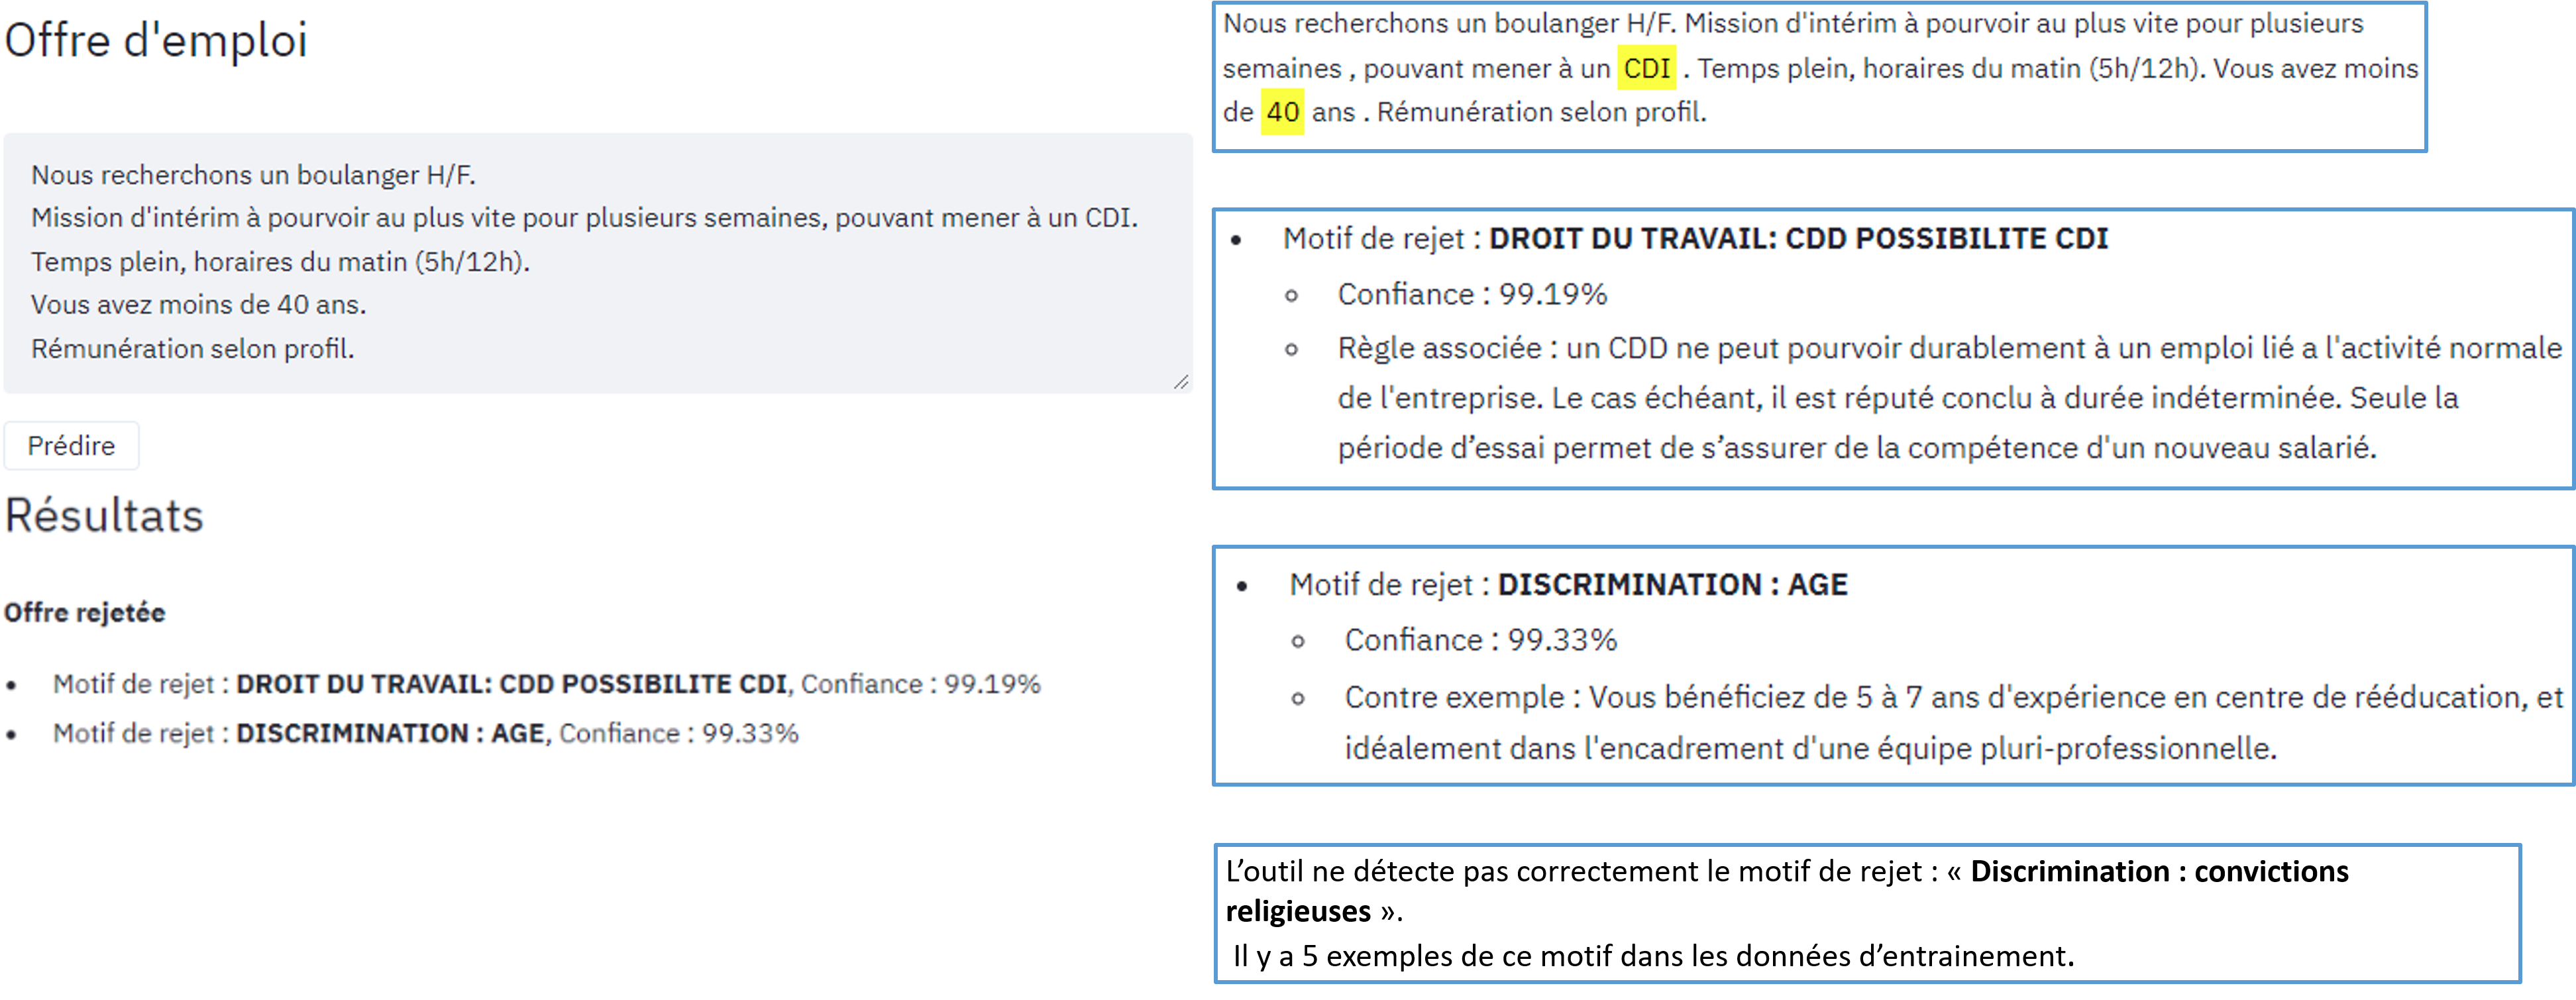
\includegraphics[scale=0.22]{Introduction/figures/format_explications.png}
    \caption{A gauche, exemple d'offre d'emploi rejetée et motifs associés. A droite, les différents formats d'explications possibles. De haut en bas : les variables, règles, exemples, et explications générées.}
    \label{fig:format_exps}
\end{figure}

% feature Based
Les explications basées sur les variables d'entrée mettent en avant une corrélation ou un lien de causalité entre une entrée et une sortie. Ces variables d'entrées peuvent être une colonne de données tabulaires, un n-gramme dans un texte, ou un pixel ou superpixel dans une image.
Ce type d'explication est très utilisé pour l'explicabilité locale, car il s'appuie directement sur une instance donnée en entrée.
Ces explications se font également par contraste : en se concentrant sur les variations menant à des décisions algorithmiques différentes.

% rule Based
Une explication peut se faire en explicitant une règle logique. Cette règle peut mettre en avant une relation de cause à effet du phénomène modélisé, ou sur une corrélation entre une variable et une sortie associée. Dans ce dernier cas, la règle est plus généralisable que l'explication basée sur les variables.
Les explications sous forme de règles peuvent notamment être extraites d'un arbre de décision, ou de contraintes appliquées au système de décision, auquel cas ce sont des explications globales. Elles peuvent aussi être des explications valides dans un périmètre local précis.

% examples Based
Les explications basées sur les exemples sont basées sur des instances réelles du phénomène modélisé. Elles évitent ainsi de s'appuyer sur des données hors distribution, adversaires ou jamais vues par le modèle lors de l'apprentissage. Lorsque c'est un contre-exemple qui est présenté, c'est à dire une instance menant à un résultat différent, alors l'explication est contrastive. Il est également possible de montrer une instance la plus différente possible mais menant au même résultat qu'une instance d'origine, on parle alors d'exemple semi-factuel.

% generated explanations
Enfin, les explications générées ne sont ni des variables, ni des règles, ni des exemples. Elles peuvent correspondre à de la documentation sur le modèle, telle que l'analyse des erreurs du modèle, ou des indications sur ses limites. Elles peuvent prendre la forme de motifs générant de fortes activations de couches d'un réseau de neurones, ou encore des textes et images générés, sans que ces derniers ne ressemblent à un exemple.
% viz montre le fonctionnement des layers~\cite{Zeiler2014}
% Artefact par classe~\cite{Simonyan2014an}
% textes et images générés~\cite{Costa2018}
% model cards :~\cite{Mitchell2019}

\subsection{Données d'applications spécifiques}
Les explications peuvent s'appliquer aux textes, images et données tabulaires. Les textes et images sont des données spécifiques, car analysés directement par les interlocuteurs humains.

Ainsi, le langage naturel est lu, entendu et parlé, et ce dès l'enfance, pour la plupart des humains. Un mot manquant ou une règle de grammaire non respectée sera alors jugée sévèrement. D'un point de vue technique, les textes sont divisibles en n-grammes. Un n-gramme est un ensemble de n entités syntaxiques consécutives, des mots ou des caractères. La figure \ref{fig:n-gramms} illustre ce concept sur un court exemple. Au-dessus de la phrase sont extraits deux bigrammes (ou 2-grammes) de lettres : ``un'' et ``hr'', parmi les 16 possibilités. En dessous sont extraits les bigrammes de mots.

\begin{figure}[htpb!]
    \centering
    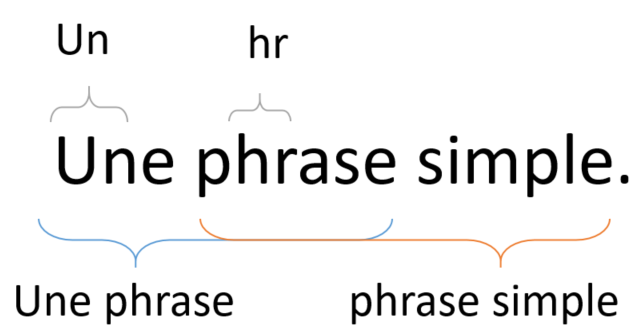
\includegraphics[scale=0.50]{Introduction/figures/n-gramm.png}
    \caption{Exemples de bigrammes de caractères en haut et de mots en bas.}
    \label{fig:n-gramms}
\end{figure}

Pour être traités par un algorithme, les textes doivent être transformés en vecteurs. Les n-grammes peuvent être utilisés directement pour vectoriser le texte, avec des méthodes d'encodage à chaud (``one-hot encoding''). Des techniques plus avancées de sac de mots telles que le TF-IDF (``Term Frequency - Inverse Document Frequency'') peuvent également être employées. Enfin, plus complexe encore, les textes peuvent être vectorisés via un plongement de mots, réseau de neurone spécialisé dans cette tâche.

Les images sont représentables par un ensemble de pixels de couleurs, sur les trois canaux rouge, vert, bleu. Techniquement une image est donc une matrice en trois dimensions : hauteur, largeur, couleur. Il est possible de représenter une image en considérant chaque pixel comme une unité. Les pixels peuvent également être rassemblés par blocs, selon leur similarité. Ces blocs sont des \textit{superpixels}. Ils permettent de découper l'image en blocs porteurs de sens. La figure \ref{fig:illustrations} montre deux images avec des explications au niveau des pixels et superpixels.

\begin{figure}[htpb!]
    \centering
    \begin{subfigure}[b]{0.44\textwidth}
       \centering 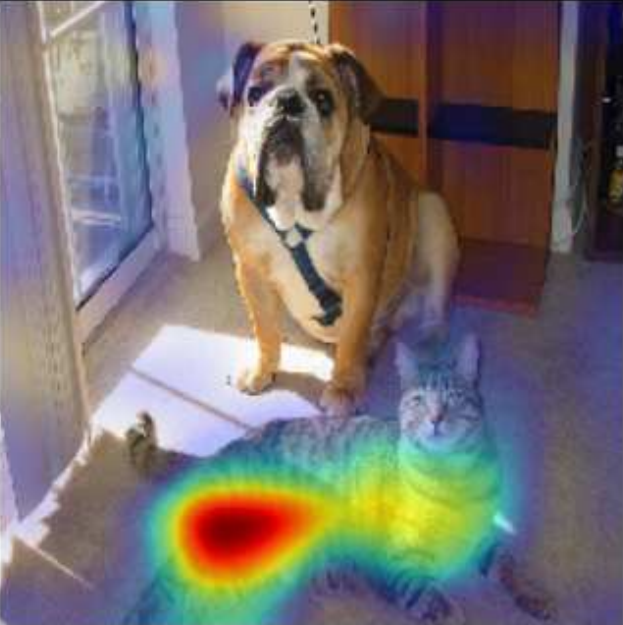
\includegraphics[width=\textwidth]{Introduction/figures/grad-cam.png}
       \caption{Explication au niveau des pixels avec la méthode Grad-CAM~\cite{Selvaraju2017}}\label{fig:gradcam}
    \end{subfigure}
    ~
    \begin{subfigure}[b]{0.44\textwidth}
       \centering 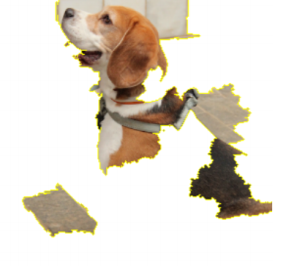
\includegraphics[width=\textwidth]{Introduction/figures/beagle_anchor.png}
       \caption{Explication au niveau des pixels avec la méthode des ancres~\cite{Ribeiro2018}}\label{fig:anchor}
    \end{subfigure}
    \caption{Différentes visualisations d'une explication sur une image.
    }\label{fig:illustrations}
\end{figure}

Enfin, les données tabulaires ont l'avantage de nécessiter moins de transformation entre leur format lisible par un humain et leur intégration dans les modèles. Toutefois, ces données sont moins naturelles à lire comparées aux textes et images.

Les données ne sont pas au choix, à moins de modifier la structure du problème initial. Toutefois elles imposent des contraintes de visualisation et possèdent leurs spécificités propres. Les portées, stratégies, formats, et les données à disposition pour générer des explications sont désormais définies.

Ces différentes caractéristiques des explications impliquent un nombre important de méthodes de génération d'explications. Ces méthodes sont adaptées à certaines caractéristiques.

\section{Comment générer une explication ?}\label{C1:generation}

Les méthodes connues sont présentées en se basant sur le découpage par stratégie, à savoir :
\begin{itemize}
    \item expliquer un modèle boîte noire via des méthodes indépendantes du modèle,
    \item observer un modèle boîte grise avec des méthodes dépendantes du modèle,
    \item concevoir un modèle transparent.
\end{itemize}

\subsection{Explications indépendantes du modèle}

Ce type de méthode a pour principal avantage de pouvoir être utilisé sur tous les modèles. Cela évite de se contraindre techniquement dans le choix d'un modèle. Les explications sont le plus souvent basées sur les variables d'entrées.
Les explications sont générées en considérant le modèle comme une boite noire. Elles relèvent donc de la corrélation plus que de la causalité.

\paragraph{Distillation de connaissance}
Une manière de rendre les modèles interprétables est de se concentrer sur des architectures simples. La distillation de connaissances dans les modèles permet d'entraîner un ensemble complexe de réseaux de neurones et transférer les structures apprises à un réseau de neurones plus simple~\cite{Hinton2015}. Instinctivement, il est tentant de se dire qu'un réseau plus simple pourrait être plus interprétable. Les auteurs de~\cite{Dhurandhar2017} proposent de mesurer l'interprétabilité comme étant le ratio entre la performance du modèle simple et du modèle complexe. En appliquant ces mesures sur un cas d'étude avec un réseau de neurones complexe et un réseau de neurones simplifié, ils en déduisent que la distillation améliore la robustesse, c'est à dire à la résistance aux attaques par modifications subtiles des entrées du modèle, au détriment de l'interprétabilité. En revanche, la distillation est également utilisée pour créer des arbres de décision~\cite{Liu2018,Wu2017} ou des arbres boostés par le gradient~\cite{Che2015} à partir de réseaux de neurones, ce qui revient à créer un module d'explication sous forme d'arbres de décisions. Si l'approche est décrite pour des réseaux de neurones, elle est applicable à d'autres modèles.

\paragraph{Importance des variables}
De nombreuses méthodes fonctionnent sur la quantification de l'importance des variables.
Les vecteurs d'explication locale quantifient l'importance de chaque variable d'entrée pour une instance donnée~\cite{Baehrens2010}. Un vecteur d'explication indique dans quelle direction changer une variable pour que le modèle change de résultat.
En observant un ensemble de vecteurs, on peut également avoir une visualisation plus globale du modèle.
Toutefois, ces vecteurs sont difficilement interprétables pour les utilisateurs, surtout dans le cas de l'analyse sémantique où la dimension est la taille du vocabulaire du corpus.

Les valeurs de Shapley donnent un aperçu de la contribution d'un élément dans un ensemble par rapport à un résultat final~\cite{Strumbelj2010}. La dimension des explications obtenues est égale à la dimension des données en entrée. Elles nécessitent donc un traitement a posteriori pour en retirer des explications claires.
Le calcul des valeurs de Shapley nécessite d'avoir accès au jeu de données d'entraînement du modèle, ce qui est une limitation forte et sous-entend un calcul éventuellement long. Pour limiter le temps de calcul, une estimation des valeurs de Shapley est donnée dans le module SHAP (``SHapley Additive exPlanation'')~\cite{Lundberg2017}.

La méthode Randomized Input Sampling for Explanation (``RISE'') masque aléatoirement des variables en entrée du modèle, pour déterminer les variables importantes~\cite{Petsiuk2018}.
Ces travaux sont approfondis pour créer des cartes de saillance (saliency maps) adaptées à chaque classe du modèle~\cite{Thakur2021}.
Les mesures d'influence quantitative des entrées donnent également le lien entre les données en entrée et les sorties d'un algorithme~\cite{Datta2016}. Cette méthode est intéressante pour sa rapidité de calcul.
La méthode COnstrained feature perturbation and COunterfactual instances (``COCO''), calcule ces poids de variables en contraignant les perturbations dans une direction choisie~\cite{Fang2021}. Malgré ces contraintes, cette méthode nécessite un long temps de calcul. Les contraintes sur les perturbations, basées sur les connaissances fonctionnelles des données, permettent également de créer des explications plus concises~\cite{Gorji2022}.


\paragraph{Approximation linéaire locale}
La méthode Local Interpretable Model-agnostic Explanations (``LIME'') mesure l'importance des variable en effectuant des perturbations aléatoires~\cite{Ribeiro2016}. LIME fonctionne par approximation linéaire du modèle autour d'une instance donnée. C'est ce modèle linéaire qui est ensuite utilisé pour générer des explications. Ces explications correspondent aux variables d'entrée qui impactent le plus la sortie du modèle. Pour l'analyse de texte, ce sont les mots du texte associés à une quantification de l'influence, positive ou négative, sur la réponse du modèle.

Dans le même article, les auteurs présentent SP-LIME, une méthode d'explication globale se basant sur les explications locales de LIME. Un ensemble d'exemples et explications locales associées est ``sélectionné judicieusement''\cite{Ribeiro2016}, étant donné un nombre $B$ prédéfini d'instances à présenter à un utilisateur.
Cette sélection s'appuie sur la recherche d'un ensemble optimal d'exemples couvrant les variables d'entrées les plus importantes. L'ensemble des exemples doit être expliqué par Lime avant d'être sélectionné par SP-Lime.
Cette méthode est intéressante car elle est généralisable au-delà de LIME~\cite{Ribeiro2018}. Par contre, elle nécessite de générer en amont toutes les explications des instances d'un ensemble de données pour pouvoir les sélectionner ensuite.

L'avantage de cette approximation linéaire est la simplicité de la création de l'explication. Toutefois il faut faire l'hypothèse forte que le modèle se comporte linéairement autour de l'instance expliquée. De même, les explications manquent de stabilité, et deux entrées très proches peuvent avoir des explications très différentes. Il est ainsi difficile pour un utilisateur humain de savoir à quel point ces explications sont généralisables.
Les perturbations de LIME sont adaptables à des domaines spécifiques, comme cela est montré dans le cadre de l'analyse d'images~\cite{Stieler2021}.


\paragraph{Ancres}\label{paragraph:anchors}
Les auteurs de LIME ont proposé une amélioration de leur méthode, les Ancres~\cite{Ribeiro2018}. En conservant l'idée d'approximation locale du modèle, les auteurs sont passés d'une approximation par un modèle linéaire à une explication sous forme de règle. L'idée est de mieux définir le contexte dans lequel l'explication générée est valable.
% Une ancre est définie comme un ensemble de variables partagé par des entrées menant à un même résultat en sortie du modèle expliqué.
Soient un modèle $f : X \rightarrow Y$, une instance $x \in X$, un résultat $y \in Y$ choisi, et une ancre $A$ associée. $A$ est une condition telle que si $x$ respecte cette condition, alors la probabilité que $f(x) = y$ est grande. L'ancre est construite de sorte à maximiser cette probabilité, il est toutefois possible que $f(x) \neq y$.
On note $D(.|A)$ l'ensemble des $x \in X$ qui respectent la condition $A$. Une ancre intéressante s'applique à un ensemble $D(.|A)$ le plus grand possible relativement à $X$.
Si les entrées sont des textes, une ancre est un ensemble de mots ou n-grammes.

Dans l'exemple illustré en Fig.~\ref{fig:anchors_domain}, le modèle étudié classe des phrases selon deux catégories : ``positive'' et ``négative''. L'instance d'origine est la phrase ``This movie is not bad'', et est classée ``positive''. L'ancre associée est la règle $A = \{not, bad\} \rightarrow Positive $.
L'ensemble $D(.|A)$  de la Fig.~\ref{fig:anchors_domain_1}, représenté par un rectangle dans la Fig.~\ref{fig:anchors_domain_2}, regroupe les entrées possédant les variables de l'ancre. Dans notre exemple, $D(.|A)$ correspond aux textes comprenant les mots ``not'' et ``bad'' de l'ensemble des variations de l'instance d'origine (ensemble $D$ de la Fig.~\ref{fig:anchors_domain}). L'ensemble $D$ est obtenu en appliquant des variations cohérentes à l'instance d'origine. Appliqué à l'exemple, cela correspond à remplacer un ou plusieurs mots de la phrase par des mots de nature similaire. Remplacer un adjectif par un autre adjectif est une variation cohérente de l'instance d'origine.

\begin{figure}[htpb!]
    \centering
    \begin{subfigure}[b]{0.22\textwidth}
       \centering 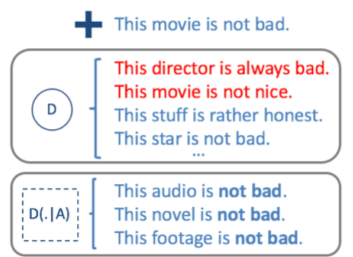
\includegraphics[width=\textwidth]{S1-Comment_evaluer_une_explication/figures/anchors_domain_1.png}
       \caption{Une entrée, ses variations $D$ et leur sous ensemble correspondant à l'ancre $D(.|A)$  }\label{fig:anchors_domain_1}
    \end{subfigure}
    ~
    \begin{subfigure}[b]{0.20\textwidth}
       \centering 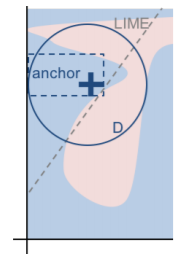
\includegraphics[width=\textwidth]{S1-Comment_evaluer_une_explication/figures/anchors_domain_2.png}
       \caption{Représentation de l'entrée (croix), et des ensembles $D$ (cercle) et $D(.|A)$ (rectangle)}\label{fig:anchors_domain_2}
    \end{subfigure}
    \caption{Textes similaires à une entrée $D$ et son sous ensemble $D(.|A)$ correspondant à l'ancre $\{not, bad\} \rightarrow Positive $. Source:~\cite{Ribeiro2018}}
    \label{fig:anchors_domain}
\end{figure}

Pour sélectionner une ancre, les auteurs choisissent de maximiser deux paramètres. Le premier est la précision, qui est maximale si les éléments de l'ensemble $D(.|A)$ ont la même sortie que l'instance d'origine. Le second est la couverture, soit la taille de l'ensemble $D(.|A)$ par rapport à l'ensemble $D$. Une ancre avec une forte précision est une explication fidèle au modèle boîte noire. Si elle a une bonne couverture, une ancre est assez généralisable.

Le travail autour des ancres met en avant la relation entre l'utilisateur et l'explication. La limite de LIME contournée par les Ancres est la difficulté pour l'utilisateur à déterminer la validité d'une l'explication donnée. Ce faisant, l'explication donnée, à savoir une règle, est également plus facile à aborder qu'un ensemble de poids comme le résultat de base de LIME.\\

Les explications indépendantes des modèles sont une première approche en considérant les modèles boîtes noires, mais il s'agit plus de mettre en avant des corrélations entre les entrées et les résultats du système.
Pour aller plus loin, il est possible de s'appuyer sur la structure du modèle pour générer des explications. La \textit{boîte noire} devient alors une \textit{boîte grise}.

\paragraph{Génération de contre-exemples}
% basé sur les perturbations
Les méthodes basées sur la perturbation telles que LIME~\cite{Ribeiro2016} et RISE~\cite{Petsiuk2018} créent des données hors distribution (\textit{out of distribution}, OOD). Ces échantillons OOD peuvent être mal classés par les modèles, mais peuvent aussi être assez inhabituels pour les utilisateurs finaux, perdant ainsi la clarté des explications. Ceci est particulièrement vrai dans le domaine du langage naturel, où le texte OOD devient très rapidement dénué de sens. Cette déviance par rapport à la distribution originale des données peut être mesurée~\cite{Qiu2021}.
% contraintes sur les perturbations
Des travaux tentent de contraindre les perturbations, en veillant à ce que les données générées soient cohérentes avec la distribution des données d'apprentissage. Cela peut être réalisé en trouvant le meilleur masque de perturbation~\cite{Chang2019} et en remplissant ce masque de la meilleure façon possible pour créer une entrée cohérente~\cite{Agarwal2020}.


% GANs
Pour aller plus loin, des entrées cohérentes peuvent être générées directement via des Réseaux antagonistes génératifs (Generative Adversarial Networks, GAN), en produisant des exemples factuels, des exemples semi-factuels et des exemples contrefactuels~\cite{Kenny2021,Charachon2021}. Ces points de données générés sont similaires à des données d'entraînement par conception, évitant la plupart des problèmes d'OOD, selon les performances du GAN. De plus, ces exemples aident les utilisateurs finaux à reconstruire un modèle mental, c'est à dire une représentation mentale du modèle. En effet, ils rendent tangibles les limites de décision, situées entre les exemples semi-factuels et contrefactuels. La mise en évidence du delta nécessaire pour franchir cette frontière peut être obtenue en calculant la différence entre les instances factuelles et contrefactuelles~\cite{Charachon2021}.

% Sobriété
Cependant, le gain en explicabilité apporté par certaines méthodes de pointe se fait au détriment du temps de calcul, et de la sobriété énergétique. A titre d'illustration, citée par~\cite{Chang2019}, une approche d'explication avec un masque de perturbation cohérent peut prendre ``environ une minute sur un seul GPU pour terminer une image''.

% SVM ?


\subsection{Explications dépendantes du modèle}

Les explications dépendantes du modèle sont basées sur l'observation des paramètres du modèle après son entraînement. Cette observation, pour conserver la métaphore de la boite noire, revient à ouvrir cette boite et regarder à l'intérieur. Les explications sont alors plus fidèles au fonctionnement du système étudié que les méthodes indépendantes du modèle. Toutefois, cette approche contraint fortement le choix du modèle.

\paragraph{Réseaux à convolutions}
Dès 2013, des travaux sur les réseaux de neurones proposent des visualisations de leur fonctionnement, dans le cadre de la classification d'images. Dans~\cite{Zeiler2014}, les auteurs proposent de mieux appréhender le fonctionnement des réseaux à convolution (Convolutionnal Neural Networks, CNN), par une visualisation directe des motifs d'activation des neurones par couche. Ils utilisent pour cela un réseau de neurones appelé \textit{Deconvolutionnal Network}. Ils obtiennent des motifs reconnus par chaque couche, motifs simples sur les couches basses et plus semblables aux classes détectées sur les couches hautes. Les auteurs vérifient également le comportement de leur modèle en masquant certaines parties des images et en observant les éventuelles variations de classification induites.

Toujours sur les CNN, la méthode de cartographie d'activation de classe, (Class Activation Mapping, CAM)~\cite{Zhou2016} est proposée. Elle permet de générer des cartes de chaleur des endroits de l'image aidant à la détection d'une classe en particulier.   .
La méthode Grad-CAM~\cite{Selvaraju2017} mélange les visualisations à celles de~\cite{Springenberg2015,Zeiler2014}, afin d'obtenir les parties de l'image ainsi que les motifs précis permettant la classification (Fig~\ref{fig:gradcam}).
Ces travaux sont repris par ~\cite{Chattopadhay2018} pour donner l'amélioration \textit{Grad-CAM++}.
Dans la continuité de cas travaux, des concepteurs ont été associés à ces trois méthodes~\cite{Qian2022}. Un concepteur est un motif de changements d'états de neurones. Les auteurs proposent grâce aux concepteurs de prendre en compte les éléments en faveur et en défaveur de la classification. Toutefois, les cartes de chaleur issues de cette méthode sont plus diffuses.
Des travaux sont également effectués sur les cartes de saillances (saliency maps) des images~\cite{Simonyan2014}. Ces travaux permettent d'avoir une indication fidèle du fonctionnement du modèle. Ces techniques sont plutôt orientées analyse d'image.

\paragraph{Long-Short Term Memory (LSTM)}
Dans la même philosophie, les auteurs de~\cite{Karpathy2016} essaient de comprendre les forces et les limites des réseaux de neurones de type LSTM, appliqués à l'analyse de textes.
Pour leur analyse, ils génèrent des visualisations sur des motifs spécifiques dans les données entraînant les activations de certaines cellules. Un exemple donné par les auteurs et présenté en figure~\ref{fig:lstm_quotes} concerne l'activation de certaines cellules en fonction des caractères rencontrés dans un texte. La visualisation met en évidence la détection du texte entre guillemets.

\begin{figure}[htpb!]
\centering
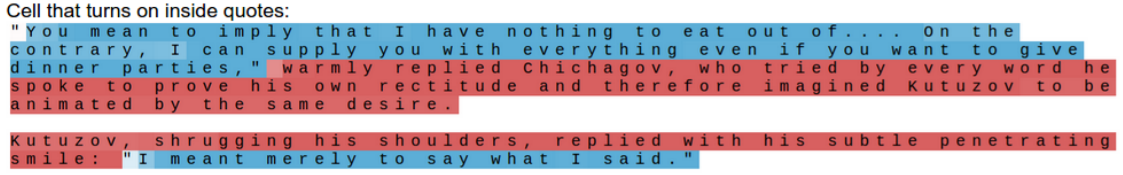
\includegraphics[width=\textwidth]{S1-Comment_evaluer_une_explication/figures/lstm_quotes_activation.png}
\caption{Activation d'une cellule en fonction des guillemets dans le texte. Source :~\cite{Karpathy2016}}
\label{fig:lstm_quotes}
\end{figure}

Ce type de réseau de neurones est largement utilisé dans l'analyse sémantique.
Les visualisations peuvent donner une idée précise du fonctionnement du modèle. Toutefois, elles sont complexes ou nécessitent un travail de recherche et d’analyse, d’autant plus si on considère chaque cellule.
Pour donner un ordre d'idée, des structures de LSTM de la littérature peuvent avoir 300~\cite{Lin2017} ou encore 512~\cite{Karpathy2016} cellules. Il convient alors de toutes les explorer pour trouver, pour une petite partie d'entre elles, des activations significatives.
Si ce type d’approche permet de mieux comprendre les indices utilisés par le réseau, il ne s’agit pas forcément d’une explication de la décision finale. L'inspection neuronale profonde (Deep Neural Inspection, DNI) repose sur les activations de la couche d'états cachés d'un LSTM de taille restreinte, afin de vérifier le respect de fonctions hypothèses définies par des experts des données, telles que la recherche d'éléments spécifiques dans les données : ponctuation pour du texte, couleurs pour les images, etc.~\cite{Sellam2019}.



\paragraph{Décomposition du modèle}
La décomposition pixel par pixel (\textit{Pixel-Wise Decomposition}, PWD) est une stratégie permettant d'expliquer les résultats d'un classifieur d'images en créant une carte de chaleur des pixels les plus pertinents pour une prédiction donnée~\cite{Bach2015}.
Pour calculer la pertinence $R$ (\textit{Relevance}) de leurs variables d'entrée, dans leur exemple des pixels. Ils décomposent la prédiction $f(x)$ comme étant la somme des contributions des neurones de la couche précédente et appliquent itérativement cette propriété jusqu'à arriver à la couche d'entrée de leur réseau. Les auteurs décrivent deux manières d'y parvenir.
La première méthode est la propagation de pertinence couche par couche (\textit{Layer-wise Relevance Propagation}, LRP), un concept regroupant diverses solutions de décomposition respectant certains critères. La seconde est une approche basée sur la décomposition de Taylor, qui permet une approximation de la propagation de pertinence couche par couche, en s'appuyant sur le principe de décomposition de fonctions pour décomposer directement le classifieur $f$.
Ces travaux sont approfondis dans~\cite{Montavon2017} où les auteurs proposent la \textit{Deep Taylor Decomposition}, qui est une adaptation de la décomposition de Taylor, appliquée non pas au modèle entier mais à chaque fonction de pertinence $R_j({x_i})$ entre un neurone $j$ d'une couche $n$ et les neurones ${x_i}$ de la couche $n-1$.
Dans ce dernier article les auteurs illustrent leurs travaux avec des réseaux de neurones classant des images, mais ce type de méthode peut être appliqué à d'autres modèles et peut également être élargi à d'autres types d'entrées, comme les textes dans~\cite{Montavon2017}.
L'analyse des éléments du modèle peut être encore plus visuelle comme avec les graphes de flux de données intégrés à la librairie de développement de modèles Tensorflow~\cite{Wongsuphasawat2017}.
L'apprentissage profond de variables importantes (Deep Learning Important FeaTures, DeepLIFT)~\cite{Shrikumar2017} utilise la rétropropagation des contributions des neurones, similairement à la LRP~\cite{Bach2015}. Les auteurs définissent ces contributions comme positives ou négatives, relativement à une contribution de référence~\cite{Shrikumar2017}.
Il est également possible de déterminer des vecteurs concepts, permettant de proposer des exemples correspondant à des concepts sémantiques pertinents sur le plan fonctionnel~\cite{Kim2018}.

Les méthodes décrites précédemment permettent de mieux appréhender le fonctionnement des modèles, en se basant sur leurs caractéristiques respectives. Toutefois ces méthodes, dépendantes ou indépendantes du modèle, nécessitent des calculs ou de l'analyse d'un grand nombre d'éléments.
 Pour éviter cela, la dernière approche est de créer un modèle dont la structure même le rend plus transparent.

\subsection{Modèle Interprétable}
L'idée de modèle transparent est de limiter le besoin en analyse post entraînement en s'appuyant sur des structures spécifiques du modèle. De cette manière une meilleure fidélité au modèle est assurée tout en limitant les calculs et approximations.


\paragraph{Architectures simplifiées}
Dans le courant de simplification des réseaux, des expérimentations mettent en évidence l'efficacité d'architectures de réseaux de neurones simplistes mais capables de résoudre des problèmes complexes, comme le stationnement d'une voiture miniature~\cite{Hasani2018}. Ce type de réseau possède une topologie inspirée du système nerveux du ver \textit{C. elegans}. Le papier définit un réseau ainsi constitué de 12 neurones, en l'entraînant sur la tâche de stationner un robot.
En observant les activations des neurones en fonction des phases, les auteurs mettent en lumière le rôle des neurones dans chaque phase de la tâche accomplie, en mettant en évidence par exemple les neurones s'activant lorsque le robot doit tourner à droite. Ces activations sont interprétables notamment parce que le réseau est composé de peu de neurones; cela facilitant grandement l'analyse des activations. Cette approche permet ainsi de réaliser un travail similaire à~\cite{Karpathy2016}, qui analyse les activations de cellules LSTM, mais sur un nombre réduit de neurones.

Considérant la représentation de modèles sous forme de fonctions, l'approche Model Learning with Personalized Interpretability Estimation (ML-PIE) permet à l'utilisateur de choisir successivement les fonctions qui lui semblent les plus explicables,  permettant la génération d'un modèle spécifiquement adapté à leur besoin~\cite{Virgolin2021}.

\paragraph{Mécanismes d'attention}\label{paragraph:attention}
Les mécanismes d'attention dans les réseaux de neurones sont une manière de rendre les modèles directement plus interprétables\cite{Bahdanau2015}. L'attention est appliquée dans diverses architectures de réseaux, dont les transformeurs qui reposent essentiellement sur ce mécanisme~\cite{Vaswani2017, Abnar2020}. Dans~\cite{Lin2017}, les auteurs créent un plongement de mots via un réseau avec une partie LSTM et une partie basée sur l'attention. Chaque phrase est représentée par une matrice $M = AH$, où $A$ est la matrice d'attention et $H$ les états cachés de la couche LSTM. Les vecteurs d'attention $a$ composant $A$ vont se concentrer sur des aspects différents de la phrase. En sommant et normalisant (par une fonction softmax) tous les vecteurs d'attention $a$, les mots fortement considérés par le plongement ressortent avec les poids les plus forts.
Cette solution permet donc d'avoir une visualisation claire des variables importantes en entrée du réseau, en observant les paramètres du modèle. Un exemple de visualisation est présenté dans le cadre de la traduction de textes dans~\cite{Olah2016} (Fig.~\ref{fig:lstm_attention}). Elle met en avant l'inversion des mots entre l'entrée en anglais (``\textit{european economic area}'') et la traduction française (``\textit{zone économique européenne}''). La visualisation des poids d'attention est également utilisée dans~\cite{Wang2016} afin de valider l'intérêt de leur topologie de réseau, également composé d'un LSTM et d'une couche d'attention. Le principal intérêt de l'analyse de l'attention est qu'il n'y a pas besoin de calculs supplémentaires d'une métrique spécifique une fois le modèle entraîné, contrairement à~\cite{Bach2015} par exemple.

\begin{figure}[htpb!]
\centering
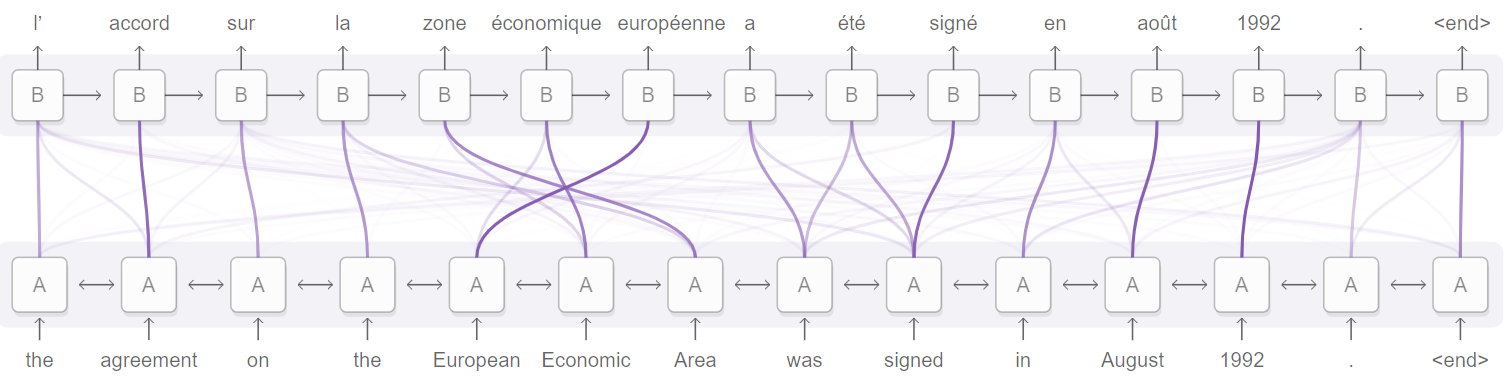
\includegraphics[width=\textwidth]{S1-Comment_evaluer_une_explication/figures/lstm_attention.png}
\caption{Visualisation de l'attention pour une tâche de traduction. Source:~\cite{Olah2016}}
\label{fig:lstm_attention}
\end{figure}

Un modèle peut également utiliser l'attention pour enrichir les données d'apprentissage. Une méthode possible est d'associer les éléments d'attention à des prototypes de données connus qui permettent la prise de décision~\cite{Barnett2021}. Le modèle est ainsi basé sur le raisonnement humain. Une autre façon de faire consiste à superposer des données et des cartes d'attentions issues de l'attention visuelle d'humains effectuant la même tâche que le modèle à entraîner~\cite{Obeso2022}.
Des mécanismes similaires ont été développés sur les modèles linéaires généralisés (Generalized Linear Models, GLM) afin d'en extraire des poids d'attention~\cite{Richman2021}.

\paragraph{Génération d'explications}
Certains systèmes peuvent également générer d'eux même des explications autour d'une décision. C'est le cas de~\cite{Costa2018} où les explications d'un système de recommandation sont générées sous forme de critiques d'utilisateurs (``\textit{I wouldn’t recommend it.}'') via un LSTM. Le principe de l'expérimentation est de reconstruire une critique que produirait un utilisateur avec un texte le plus naturel possible. Les auteurs évaluent leurs explications avec des métriques de lisibilité de textes tel que le score \textit{Flesch-Reading-Ease}. Si le système de recommandation n'est pas nécessairement un réseau de neurones, un système similaire peut être appliqué à tout système de prédiction basé sur des textes.
Ces explications générées peuvent être plus globales, comme les cartes de modèles, reprenant un ensemble structuré d'informations concernant un modèle~\cite{Fang2020}.

D'autres architectures de modèles apprennent des concepts non supervisés dans les données. Les réseaux de neurones auto-explicatifs (Self-Explaining Neural Network, SENN) utilisent l'architecture encodeur-décodeur pour apprendre ces concepts~\cite{AlvarezMelis2018}. Certains montrent l'activation neuronale associée à des éléments de concept, tels que les couleurs dans le cadre de l'analyse d'images~\cite{Barberan2022}.
Ces concepts peuvent être supervisés, c'est le cas des modèles de goulots d'étranglement conceptuels (Concept Bottleneck Models, CBM), qui apprennent à associer une entrée à un ensemble de concepts, présents dans les données d'entraînement, puis les ensembles de concepts à une classe~\cite{Koh2020}.
Une fusion des concepts supervisés et non supervisés de~\cite{AlvarezMelis2018,Koh2020} intègre à la fois l'expertise métier et la découverte de nouveaux concepts~\cite{Sawada2022}.
Similairement aux concepts, des prototypes de granularité modulable peuvent être présentés, issus des motifs présents dans les données d'entraînement du modèle~\cite{Uehara2020}. Le dictionnaire de prototypes associés peut être directement appris par le modèle, ~\cite{Uehara2021,Yun2021}. Dans le cadre de l'analyse des séries temporelles, la méthode eXplainable Representation of Complex System Behavior (XR-CSB) extrait ces concepts correspondant à des états~\cite{Kaadoud2022}. XR-CSB permet de générer des explications sous la forme d'automates à états.


Les principales méthodes d'explicabilité ont été abordées, proposant un aperçu de la multiplicité des propositions de la communauté. Chaque méthode possède ses avantages et inconvénients. La section suivante couvre l'état de l'art de l'évaluation de ces méthodes.


\section{Comment évaluer une explication ?} \label{C1:evaluations}

Évaluer les méthodes d'explicabilité n'est pas systématiquement réalisé dans la littérature. Toutefois de nombreuses méthodes sont présentées dans ce chapitre, associées aux points qu'elles permettent d'évaluer.

Les méthodes d'évaluation sont basées sur des mesures tirées des explications elles même, ou s'appuient sur le ressenti utilisateur ou l'impact d'une explication dans une tâche~\cite{Ayyar2021, Dodge2020}. Le choix d'une méthode adaptée rend compte non seulement de la qualité d'une explication mais aussi de son adéquation avec les objectifs de l'outil global dans la réalisation d'un acte métier.

Cette section présente les différentes méthodes d'évaluation des explications, à l'état de l'art.
% Plan
La section \ref{C1:proprietes} définit les propriétés souhaitables pour une explication, recoupant et regroupant les noms parfois différents dans la littérature. Il vise à aider la sélection d'une ou plusieurs propriétés à maximiser, ce qui guidera le choix d'une méthode d'évaluation par la suite.
La section \ref{C1:utilisateurs} définit les avantages et inconvénients de deux types de protocoles, ceux faisant appel à des utilisateurs et ceux qui s'en détachent. L'intégration d'humains dans un protocole expérimental apportant un travail conséquent, ce choix doit être réfléchi et motivé.
Les sections \ref{C1:ev_obj} et \ref{C1:ev_subj} présentent les méthodes d'évaluation de la littérature, les liant aux propriétés qu'elles permettent d'évaluer.
Enfin, la section \ref{C1:debat} met en avant les challenges du domaine dans le lien entre évaluation technique et évaluation humaine.


\subsection{Propriétés souhaitées} \label{C1:proprietes}

% objectif
Les propriétés souhaitées des explications sont nombreuses. Cette section les regroupe en harmonisant les notations de l'état de l'art quand cela est possible.
% Plan
Dans un premier temps, les propriétés qui conviennent à toutes les explications seront citées avant d'être détaillées.

Les propriétés des explications sont souvent appelées avec des noms variables dans la littérature. Toutefois, il est possible de les regrouper sous des adjectifs suffisamment génériques.

\paragraph{Fidèle}
La fidélité correspond à la capacité d'une explication à être en accord avec le phénomène ou modèle expliqué~\cite{Guidotti2018,Lundberg2017,Lakkaraju2019,Ribeiro2018,Hoffman2018,Liu2021,Ciravegna2020}.
Pour~\cite{Codella2019} cela signifie qu'elle est argumentée ; elle s'appuie sur des éléments vérifiables par le receveur. Pour une tâche de classification d'images de chien, cela signifierai souligner des éléments que le receveur sait être différenciant : forme des oreilles, du museau, etc. Pour~\cite{Petsiuk2018, DeYoung2019} elle comporte donc les éléments minimaux permettant la prise de décision.

\paragraph{Interprétable}
L'interprétabilité d'une explication est une notion plus complexe. Pour~\cite{Guidotti2018,Virgolin2021,Lakkaraju2019} cela correspond à la taille d'un modèle élève générant les explications, donnant ainsi une explication de taille raisonnable.~\cite{Ribeiro2016} abonde dans ce sens en indiquant qu'une explication interprétable possède un nombre limité d'éléments et s'appuie sur des notions adaptées à son receveur. Pour~\cite{Gilpin2018} cela signifie que l'explication est suffisamment simple pour être comprise. Il est ainsi possible de découper l'interprétabilité en trois propriétés plus spécifiques : la concision, la complétude et l'adaptation.

\subparagraph{Concise}
Une explication concise comporte un nombre limité d'éléments. Le receveur n'est pas noyé par la quantité d'informations. Si de nombreux travaux y font référence~\cite{Ribeiro2016,Petsiuk2018, Poppi2021,Lakkaraju2019,Zafar2021a},~\cite{Miller2017} va plus loin, mettant en avant le fait que les receveurs ont une forte tendance à favoriser les explications les plus courtes.
\cite{Gilpin2018} met en garde contre le biais humain qui, en favorisant les explications courtes, risque de préférer des systèmes d'explications persuasifs plutôt qu'interprétables. Ces systèmes s'appuient alors sur des connaissances et préférences des receveurs, quitte à être moins fidèles~\cite{Herman2017}.

\subparagraph{Auto-explicative}
Une explication est auto-explicative lorsqu'elle ne nécessite pas de connaissances supplémentaires pour être comprise~\cite{Codella2019,Gilpin2018}. Par exemple, une équation sera facilement interprétable pour un expert de la donnée, mais pas pour un receveur n'ayant pas l'habitude de manipuler ce format d'information~\cite{Ribeiro2016}. Elle comporte donc tous les éléments nécessaires à sa compréhension sans qu'il soit nécessaire de les détailler~\cite{Hoffman2018}.

\subparagraph{Adaptée aux receveurs}
Une explication adaptée aux receveurs est conçue dans un vocabulaire connu de ces derniers, par exemple en intégrant le vocabulaire spécifique à la tâche ou domaine métier associé~\cite{Codella2019}.
\cite{Dam2018, DeYoung2019} abondent en ce sens, estimant qu'elle pourrait ressembler aux explications que fourniraient des humains qui auraient la même tâche. Dans cette même dynamique mais spécifique au TALN, les travaux de~\cite{Zafar2021a} montrent que les utilisateurs ont une préférence pour les explications de textes basées sur des phrases plutôt que sur des mots.

\paragraph{Représentative}
Une propriété associée est la non-ambigüité, définie par~\cite{Lakkaraju2019} pour un ensemble de règles, comme le respect à la fois d'une bonne couverture des règles, et d'un faible empiètement des règles les unes entre les autres~\cite{Lakkaraju2019}.

\paragraph{Utile}
Enfin, l'utilité des explications met en avant son intérêt pour les receveurs selon leurs attentes~\cite{Miller2017,Hoffman2018}. Si le receveur est un scientifique des données, manager ou régulateur, cela correspond à détecter des biais~\cite{Gilpin2018}.
Pour un expert du domaine ou une personne concernée par l'usage du modèle, l'utilité peut être une meilleure représentation mentale du comportement du modèle, le modèle mental~\cite{Arrieta2020,Ribeiro2018,Dam2018,Mohseni2021a}, notamment en détectant mieux ses erreurs~\cite{DoshiVelez2017}.

Pour un utilisateur cela peut l'amener à améliorer sa performance dans l'acte métier associé, ou aller plus vite~\cite{Ribeiro2018, Dhurandhar2017,Gilpin2018,Janssen2020,Mohseni2021a}. Pour tout utilisateur, l'utilité crée ou améliore sa confiance dans le modèle~\cite{Hoffman2018,Mohseni2021a}. Dans cette même optique,~\cite{Rasouli2022} propose de favoriser la mise en avant de critères actionnables, c'est à dire ceux sur lesquels l'utilisateur peut agir ou conseiller une action.
\vspace{1cm}

Il est difficile de maximiser chaque propriété, notamment parce que certaines sont incompatibles. Ainsi l'auto-explicabilité empêche la concision. Pour chaque projet, un ensemble de propriétés sur lesquelles doit se porter l'effort peut être défini. Ces propriétés étant définies, les sections suivantes définissent les modalités d'évaluation du respect de celles-ci. Dans la section \ref{C1:utilisateurs} est discutée la présence ou non des utilisateurs humains lors de l'évaluation des explications.

\subsection{\'Evaluation avec ou sans utilisateur} \label{C1:utilisateurs}

Les modalités d'évaluation des explications sont dépendantes à la fois des contraintes du projet : temps, argent, disponibilité des différents acteurs, mais aussi des propriétés souhaitées, vues en section précédente. Nous présentons les trois niveaux d'évaluation de la littérature : avec des utilisateurs réels, avec des systèmes simulant le comportement des utilisateurs, ou sans utilisateurs, ni réels ni simulés.

\paragraph{Avec des utilisateurs réels} \label{C1:utilisateurs_reels} % utilisateur ou autre nom ?
% Pourquoi
L'évaluation avec utilisateur permet de valider la bonne adéquation entre l'explication et son receveur. Elle assure notamment que les propriétés d'interprétabilité et d'utilité sont valides.
% Comment
\cite{DoshiVelez2017} divise explicitement les évaluations avec utilisateurs en deux types, observés dans la littérature. Ces évaluations sont :
\begin{enumerate}
    \item l'\'evaluation applicative,
    \item l'\'evaluation humaine
\end{enumerate}

% \item \'Evaluation applicative
Pour l'évaluation applicative, les conditions d'utilisation du modèle doivent être les plus proches possible de la réalité. L'évaluation porte alors sur la compréhension et la préférence de l'utilisateur recevant l'explication. Le profil de cet utilisateur doit correspondre à celui ou ceux auxquels sont destinés les explications. Il est ainsi possible de demander à effectuer l'action métier, avec et sans explications, ou avec des explications différentes, et comparer les performances et la vélocité de l'utilisateur~\cite{Dam2018}. Une évaluation similaire consiste à demander aux utilisateurs de donner une explication au même format, et comparer les deux. Toutefois elle nécessite de travailler sur des modèles simples, elle est donc moins adaptée à l'apprentissage profond~\cite{Lundberg2017, Dam2018}.

% \item \'Evaluation humaine, sur des tâches simples
L'évaluation humaine se fait sur des tâches simplifiées, et non l'acte métier cible. De même elle ne nécessite pas de faire appel spécifiquement au public cible des explications, ce qui est intéressant lorsque ce public est composé d'experts peu disponibles. Une tâche simplifiée peut être :
\begin{itemize}
    \item la comparaison de paires d'explications~\cite{Lakkaraju2019,Dam2018},
    \item la comparaison de modèles simples tels que des petits arbres de décision\cite{Allahyari2011},
    \item l'évaluation qualitative d'une explication pour un cas fonctionnel connu~\cite{Kaadoud2022},
    \item retrouver le même résultat que le modèle, à l'aide de l'entrée et l'explication associée~\cite{Ribeiro2018, Dam2018, Zafar2021a,Lim2009},
    \item sélectionner le ``meilleur modèle'' selon les résultats et explications associées~\cite{Ribeiro2016}.
\end{itemize}
Ces évaluations se font avec un ordre de grandeur de une à plusieurs dizaines d'humains participant : 33 pour~\cite{Lakkaraju2019}, 15 pour~\cite{Zafar2021a}. Quelques expérimentations sont menées à plus grandes échelles comme celle de~\cite{Allahyari2011} dont qui fait appel à 100 personnes, ou celle de~\cite{Lim2009} qui rassemble 158 personnes.

% Avantages
Présenter les explications à un receveur permet de s'assurer de la bonne adéquation entre ce dernier et le format d'explication proposé. Ce type d'évaluation est le plus proche des conditions réelles d'usage des explications, et est donc le plus précis. C'est la seule modalité d'évaluation qui permet de vérifier que le vocabulaire est adapté.
% Inconvénients
Cette précision a un coût non négligeable~\cite{Dam2018, DoshiVelez2017}. Ce type d'évaluation nécessite également de prendre du temps, notamment pour récolter les évaluations des receveurs. Dans le cas où des professionnels sont requis, iels sont parfois très peu disponibles : experts, médecins etc. Ces évaluations sont également sensibles aux biais humains, avec une préférence pour les explications courtes, qui ressemblent à celles que fournirait un humain~\cite{Petsiuk2018,Miller2019,Gilpin2018}.


\paragraph{Avec des utilisateurs simulés}
% Pourquoi
Il est également possible d'évaluer une explication pour son niveau d'informations et son adéquation avec l'acte métier associé. C'est alors la performance au regard de la tâche à accomplir qui est mesurée.
% Comment
Pour mesurer cette performance, quand les utilisateurs sont peu disponibles, il est possible de les remplacer par des algorithmes simulant leur comportement.
% Les utilisateurs réels vus en section précédente sont des humains, avec des expertises pouvant être variées.
Les utilisateurs simulés sont des modèles plus ou moins complexes, tels que des forêts aléatoires ou des réseaux de neurones~\cite{Ribeiro2018}. Ces utilisateurs simulés peuvent effectuer, à l'instar des utilisateurs réels, des tâches complexes ou simplifiées. Il est ainsi possible d'entraîner un classifieur qui va prédire une classe en s'aidant de l'explication pour la retrouver~\cite{Ribeiro2016, Ribeiro2018, Dhurandhar2017}, ou encore choisir le meilleur modèle, grâce aux explications~\cite{Ribeiro2016}.

% Avantages
Ce type d'expérimentation est intéressant dans la mesure où son coût est moindre comparé aux expérimentations avec utilisateurs réels. En particulier, si les utilisateurs ciblés sont des experts, les utilisateurs simulés ont l'avantage de ne pas être limité en nombre ou en quantité de données d'expérimentation traitées. Ils permettent de rester proche de l'acte métier, en simulant cet acte par exemple. Enfin, ils permettent une bonne reproductibilité, facilitant les comparaisons entre méthodes, contrairement aux expériences avec des utilisateurs réels.
% Inconvénients
Toutefois, il n'est pas possible de valider le vocabulaire ou l'acceptation d'un système comme c'est le cas avec des utilisateurs réels.
% On s'appuie sur des modèles pour valider d'autres modèles, potentiellement mal perçu, peut aussi ajouter des biais

\paragraph{Sans utilisateurs} \label{C1:no_user}

% Pourquoi
Enfin, il est possible de valider les propriétés des explications sur de larges jeux de données, sans recourir aux utilisateurs. Dès lors que la propriété est mesurable (définie par une équation), elle peut alors être directement évaluée et comparée.

% Comment
Les évaluations sans utilisateurs se font par la mesure d'une propriété. La concision pourra être associée au nombre de variables remontées dans une explication basée sur ces dernières~\cite{Zafar2021a}. La fidélité pourra correspondre au taux d'erreur d'un système d'explication en regard du phénomène ou modèle qu'il doit expliquer~\cite{Lakkaraju2019}. Dans~\cite{Petsiuk2018}, les éléments constituant l'explication sont supprimés un à un de l'entrée du modèle et l'observation du changement de résultat indique la pertinence de l'explication : plus celle-ci se fait tôt, plus les éléments constituant l'explication étaient nécessaires pour mener au résultat.

% Avantages
Les expérimentations sans utilisateur ont un coût moindre, et une bonne reproductibilité. Ils sont encore plus adaptés à l'évaluation comparative que les utilisateurs simulés, car ils ne nécessitent pas l'entraînement de ces derniers.
% Inconvénients
Toutefois, ils sont dé-corrélés de l'acte métier, et doivent servir à la comparaison de propriétés formalisées mathématiquement.


Les différentes modalités d'expérimentations influent sur les types d'évaluation. La section \ref{C1:ev_obj} détaille les possibles évaluations objectives, tandis que la section~\ref{C1:ev_subj} détaille les possibles évaluations subjectives.

\subsection{\'Evaluation objective} \label{C1:ev_obj}
% Objectif
Les évaluations objectives permettent de mesurer impartialement les performances du système explicatif, ou des explications en elles-mêmes. Il se fait principalement sans utilisateurs, par la mesure de propriétés telle qu'abordée en section~\ref{C1:no_user}. Toutefois, les mesures objectives peuvent également être extraites des expériences utilisateurs.

Chaque mesure met en avant un aspect des explications, et peut permettre de valider le respect d'une propriété. Toutefois, il n'existe pas aujourd'hui une mesure universelle qui permettrait d'évaluer et comparer tous les systèmes explicatifs existants~\cite{DoshiVelez2017}.
% Objectif
Cette section présente les mesures objectives de la littérature, permettant d'évaluer les systèmes d'explications. Les mesures sont associées aux propriétés auxquelles elles sont associées.
% Plan section
Les évaluations présentées sont respectivement centrées sur l'explication et l'acte métier.

\paragraph{Centrée sur l'explication}

Lorsque le système d'explication est un modèle, les propriétés de ce modèle forment une première source de mesures objectives. C'est le cas avec LIME~\cite{Ribeiro2016}
Pour mesurer la concision du modèle, il est possible d'utiliser sa taille en tant que nombre de paramètres~\cite{Guidotti2018}.
Toutefois cette mesure ne rend pas compte de ce qu'a appris le modèle. On peut alors y associer des mesures portant sur la fidélité du modèle, caractérisée par les mesures communes en IA : exactitude ($exactitude = \frac{\#\textrm{bonnes réponses}}{\#\textrm{réponses}} $) précision etc.~\cite{Lundberg2017,Lakkaraju2019,Ribeiro2018,Hoffman2018,Liu2021}.

En se concentrant non pas sur le système d'explication mais sur les explications en elles-mêmes, il est possible de vérifier leur conformité avec des propriétés désirées. Pour une propriété, il existe parfois de nombreuses mesures dans la littérature. Chaque propriété évaluée par des mesures objectives est reprise, cette fois en détaillant les principales manières de les mesurer.

\subparagraph{Fidèle}
La mesure de fidélité des explications est rapidement mise en place en altérant les données d'entrée à partir des explications~\cite{Samek2016,Samek2017,Montavon2018,Schlegel2019}.
Pour~\cite{Petsiuk2018} la présence d'éléments minimaux permettant la prise de décision est caractérisée par une faible Deletion Area Under Curve (DAUC). La DAUC est l'aire sous la courbe de score de classification, pour la classe cible, lors de la suppression d'éléments de l'explication, du plus important au moins important, selon un score d'importance attribué par la méthode d'explication évaluée. Cette évaluation est particulièrement adaptée aux cartes de saillances sur les images. Une instance dénuée des éléments expliquant le plus une classe sera dans cette logique, très rapidement détectée comme n'appartenant pas à cette classe. Similairement,~\cite{Petsiuk2018} présente l'Insertion Area Under Curve, (IAUC). L'IAUC est caractérisée par l'aire sous la courbe de score de classification, pour la classe cible, lors de l'insertion d'éléments de l'explication.
\cite{Gomez2022} propose une amélioration de la DAUC et l'IAUC qui favorise cette propriété: la corrélation de suppression (Deletion Correlation, DC) et la corrélation d'insertion (Insertion Correlation, IC), qui prennent en compte les pondérations des éléments de l'explication. Cette modification permet de pénaliser les explications mal calibrées par rapport au modèle expliqué. Les explications courtes sont pénalisées si le modèle s'appuie sur un nombre élevé d'éléments, et favorisées si le modèle s'appuie sur un nombre limité d'éléments.
Pour~\cite{Adebayo2018}, la fidélité est caractérisée en mesurant l'impact des changements de paramètres du modèle sur l'explication reçue.

\subparagraph{Concise}
La concision est mesurée par la taille d'une explication ~\cite{Ribeiro2016, Poppi2021,Lakkaraju2019,Zafar2021a}, une explication concise comporte un nombre limité d'éléments.


\subparagraph{Adaptée aux receveurs}
Pour vérifier, comme le préconisent~\cite{Dam2018, DeYoung2019} qu'une explication ressemble aux explications que fourniraient des humains qui auraient la même tâche, il est possible d'utiliser des mesures telles que l' intersection sur l'union (Intersection over Union, IOU)~\cite{DeYoung2019}. Le calcul de l'IOU donne un score de similarité de 0 à 1, et se calcule, pour deux ensembles A et B : $IOU_{AB} = \frac{A\cap B}{A\cup B}$. Une IOU de 1 signifie que deux ensembles sont identiques. Cette métrique est utilisée dans~\cite{Bau2017} pour évaluer les explications sur les images. Si seules quelques explications sont possibles, le cas peut être considéré comme un problème de classification, et les mesures de précision habituelles peuvent être utilisées~\cite{Codella2019}.

Pour mesurer la clarté et lisibilité des explications sous forme de textes, le score \textit{Flesch-Reading-Ease} peut être appliqué~\cite{Costa2018}. Il est calculé via la formule suivante :
\begin{equation}
    FRE = 206,835 - 84,6 * M - 1,015 * P
\end{equation}
où le terme $M = \frac{\#\textrm{nombre de syllabes}}{\#\textrm{mot}}$ correspond à la longueur moyenne d'un mot, en nombre de syllabes, et $P = \frac{\#\textrm{mots}}{\#\textrm{phrases}}$ et la longueur moyenne d'une phrase en nombre de mots. Les coefficients sont déterminés de façon totalement empirique, de sorte qu'un texte facilement lisible obtienne un score proche de 100, et un texte expert soit associé à un score proche de 0.
Toutefois ce score est spécifique à l'anglais et il n'existe pas d'équivalent français faisant figure de référence.

\subparagraph{Représentative}
La représentativité ou couverture d'une explication $A$ est définie dans~\cite{Ribeiro2018} par l'équation
\begin{equation}
    \textrm{cov}(A) = \mathbb{E}_{D(z)}[A_{(z)}]
\end{equation}.
La représentativité de $A$ est donc la probabilité $\mathbb{E}$ qu'elle s'applique aux éléments $z$ d'un ensemble d'instances $D$. En d'autres termes, $A$ est représentative si elle est valide pour un grand nombre d'éléments de $D$ où elle est appliquée.

Dans le cadre de la représentativité d'une règle,~\cite{Lakkaraju2019} considère la couverture comme le nombre d'éléments concernés par une règle. %, et superposition des règles comme le nombre de règles additionnelles pour un élément, soit $superposition = max(0,\#règles-1)$


\paragraph{Centrée sur l'usage}
Au-delà de l'explication en elle-même, l'évaluation peut porter sur l'intégration de l'explication et son intérêt pour l'acte métier ou l'usage final du modèle expliqué. Puisque les mesures présentées sont objectives, il n'est pas question ici de préférence utilisateur, mais de critères de performance ou de réussite pour le cas d'usage. Ainsi, cette section se rapporte à la propriété d'utilité vue en section \ref{C1:proprietes}.

% modèle mental
% créer leur propre représentation mentale de ce modèle. Cela leur permet de se faire une idée de la capacité du modèle à classer une instance donnée dans une classe donnée.
Pour un expert du domaine ou une personne concernée par l'usage du modèle, l'utilité peut être une meilleure représentation mentale du comportement du modèle, aussi appelée modèle mental~\cite{Arrieta2020,Dam2018,Mohseni2021a}. Cette représentation peut être mesurée au travers de la précision humaine, soit la capacité d'un humain à anticiper le comportement d'un modèle sur des instances inconnues. La précision humaine est alors définie comme étant la proportion d'instances pour lesquelles les utilisateurs arrivent à anticiper le résultat du modèle~\cite{DoshiVelez2017}. Cette mesure de précision peut aussi être effectuée avec des utilisateurs simulés, rendant l'expérience reproductible~\cite{Ribeiro2018}.
Pour les utilisateurs réels, la bonne représentation du modèle mental passe aussi par sa couverture, correspondant à la part de prédictions pour lesquelles l'utilisateur choisit de proposer une réponse autre que ``je ne sais pas'' lorsqu'on lui demande d'anticiper le résultat du modèle~\cite{Ribeiro2018}.

Dans~\cite{Iyer2018}, les utilisateurs doivent prédire la suite d'une vidéo selon quatre possibilités. Un groupe reçoit l'entrée du modèle sous forme d'images, et un second groupe reçoit une explication sous forme de carte de saillance de ces mêmes images. Les participants doivent alors prédire la sortie du modèle. Considérant les réponses des utilisateurs comme des résultats de classificateurs binaires, les auteurs calculent une courbe ROC (\textit{Receiver Operating Characteristic}, ou caractéristique de fonctionnement du receveur), son aire sous la courbe donnant la mesure du succès de leurs cartes de saillance. % 40 participants

Les auteurs de~\cite{Dam2018} proposent une méthode d'évaluation dans laquelle les humains doivent copier la décision d'un modèle en ayant une instance et son explication. Il est aussi possible de présenter aux utilisateurs, une instance, la décision $y$ et l'explication associées, et leur demander comment iels changeraient le modèle pour avoir une décision donnée $\bar{y} \neq y$. Cette tâche nécessite à l'utilisateur de bien comprendre le modèle.

% performance
Pour un utilisateur, l'explication peut l'amener à améliorer sa performance dans l'acte métier associé. Dans les travaux de~\cite{Janssen2020}, la tâche des utilisateurs est d'accepter ou refuser des dossiers de demande d'asile et permis de séjour pour les Pays Bas. Elle est présentée sous forme de texte décrivant la situation, reprenant des données tabulaires.
Deux types d'explications sont proposés ici : un basé sur des règles (\textit{``Valid reason for fleeing the country''}, ``la raison pour fuir le pays est valide''~\cite{Janssen2020}), l'autre donnant un pourcentage de confiance du modèle pour un cas similaire.
Le nombre moyen de dossiers correctement traités augmente si les participants, novices ou experts, reçoivent une recommandation accompagnée d'une explication avec le dossier.

% vitesse, doute, confiance
L'utilité peut également rendre l'utilisateur plus rapide pour effectuer sa tâche. Il est alors possible de mesurer sa vélocité avec et sans explication, et mesurer le gain de temps~\cite{Ribeiro2018,Zafar2021a}. \cite{Ribeiro2018} propose cette évaluation sur la classification de données tabulaires, avec des explications basées sur les variables.  %  Il permet d'avoir une idée de l'assurance de l'utilisateur lorsqu'il répond.

% critères actionnables
Enfin,~\cite{Rasouli2022} propose la mise en avant de critères actionnables dans les explications. Pour des données tabulaires, il s'agit de variables dont les valeurs peuvent être changées, correspondant à des éléments logiquement actionnables dans la réalité. Cette contrainte est directement intégrée dans sous la forme de contraintes et de coûts. Dans leur exemple, l'âge d'une personne est contraint à ne pas pouvoir diminuer.

% conclusion
Les différentes évaluations objectives permettant d'évaluer les explications, selon les propriétés souhaitées, ont été passées en revue. Ces mesures permettent la comparaison de système d'explications sur des éléments techniques et sans tenir compte du ressenti humain. La section suivante présente les mesures subjectives, axées cette fois sur la préférence des utilisateurs.

% Liu2021 mesures d'évaluations :
% Linéaires, ne conviennent pas à du DL :
% faithfulness - évolution de perf du modèle quand on suppr des features - : en délétion, + en addition
% monotonicity : amélioration de chaque var ordonnée selon les poids d'importance
% non linéaire, convient à du DL :
% shapley MSE et corr , nécessite de calculer les GT valeurs de Shapley
% Leurs mesures ont un sens technique, mais aucun lien sémantique pour l'utilisateur, ne remplace pas les études utilisateurs, leurs travaux permettent d'affiner avant ces études.

%~\cite{Poppi2021}.
% Les auteurs constatent que les explications de la famille des CAM sont évaluées qualitativement. Ils souhaitent mettre en place une série de mesures d'évaluation. Cet ensemble doit faciliter la comparaison d'outils
% Reprennent des mesures déjà vues : Average drop, Average increase (portent tous les deux sur la confiance du modèle avec full input VS parties de l'input formant l'explication), et insertion/deletion; et expliquent que c'est peu pratique d'évaluer des méthodes avec +sieurs chiffres.
% ils proposent :
% Maximum coherency : should remove useless feature ``in a coherent way'' (cf eq2)
% Minimum complexity : as simple as possible
% minimum confidence drop : should produce the smallest drop of confidence compared to the original input (= avg drop metric)
% Et combinent le tout dans une seule mesure : average DDC

\subsection{\'Evaluations subjectives} \label{C1:ev_subj}
% subjectif = partial, personnel, jugement
Lorsque l'objectif de l'explicabilité est de favoriser l'acceptation d'un modèle par un humain, les évaluations subjectives permettent de prendre en compte la préférence des personnes recevant l'explication. Ces évaluations se font donc nécessairement avec des humains, afin de rendre compte de leur jugement. De par leur plus grande complexité de mise en place, les évaluations subjectives sont moins présentes dans la littérature, comparées à l’évaluation objective~\cite{Lakkaraju2019}.
% Avantages
Ce type d'évaluation prend en compte le lien entre l'explication et les personnes les recevant, et notamment le ressenti de ces dernières.
% inconvénients
Ces évaluations sont coûteuses et requièrent du temps~\cite{Dam2018, DoshiVelez2017}. Elles sont également sensibles aux biais humains~\cite{Petsiuk2018}.
De même, contrairement aux mesures objectives, les évaluations subjectives ne sont pas reproductibles et conviennent moins pour la réalisation d'études comparatives.
% Objectif section
Les différents types d'études comparatives sont détaillés dans cette section, et associés aux propriétés souhaitées des explications.
%Plan section
La section se divise en deux parties, une première portant sur les études des tâches réelles, et la seconde sur les tâches annexes.

\paragraph{Sur une tâche réelle}

Il est recommandé que la tâche effectuée lors de l'évaluation représente au mieux l'environnement fonctionnel dans lequel est utilisé le système créé, avec le public ciblé~\cite{Dam2018}. Ceci permet de prendre en compte le contexte inhérent aux explications et les spécificités du public ciblé. Ainsi, les auteurs de~\cite{Dam2018} proposent de mesurer la satisfaction ressentie lorsqu'une personne utilise un outil d'IA avec les explications associées pour effectuer un acte métier.

Les auteurs de~\cite{Ribeiro2018} réalisent une mesure subjective de préférence avec un questionnaire demandant à des utilisateurs quelle explication iels préfèrent entre deux systèmes explicatifs : LIME et les Ancres. De même, les auteurs de~\cite{Lakkaraju2019} effectuent la comparaison de leur solution avec LIME. % ``quelle explication préférez-vous'' (12 personnes dans l’expérimentation)

\paragraph{Sur une tâche annexe}

Lorsque le public cible n'est pas disponible, ou que l'acte métier du système d'IA n'est pas utilisable ou simulable pour les évaluations, il est possible de passer par l'évaluation sur une tâche annexe.

% copie
Une tâche annexe simple consiste à faire deviner à un humain le résultat d'un modèle d'IA. La nuance ici est qu'il n'est pas souhaité d'effectuer la tâche réelle du modèle, mais de reproduire ses bonnes comme ses mauvaises réponses.
Dans~\cite{Lakkaraju2019}, les humains reçoivent une explication d'un système d'explication parmi trois. Cinq questions sont posées pour évaluer leur compréhension du modèle dans différents sous espaces. La précision des participants est mesurée et permet la comparaison des différents outils de génération de règles.

% Préférence
Une autre évaluation consiste à demander à un humain de choisir entre deux classifieurs, l'un étant significativement meilleur que l'autre, compte tenu uniquement de leurs explications~\cite{Ribeiro2016}. L'expérimentation de~\cite{Allahyari2011} fonctionne sur le même principe en effectuant une comparaison par paires de modèles d'apprentissage automatique réputés compréhensibles : moteurs de règle, arbres de décision etc. Les participants ont les bases nécessaires pour comprendre les éléments présentés. La question posée est de dire si un des deux modèles présentés est plus compréhensible que l'autre. Le retour des participants se fait via une échelle de Likert, où l'échelon 1 correspond à une perception égale des modèles, et l'échelon 9 un des deux modèles est bien plus compréhensible que l'autre. La tâche de l'utilisateur n'est plus l'acte métier mais la sélection du meilleur outil pour accomplir cette dernière. Ces évaluations sont appropriées lorsque l'objectif est d'améliorer l'acceptation d'un modèle.

% Conclusion
Les évaluations subjectives, basées sur la préférence humaine, ont été décrites aussi bien sur des tâches réelles que sur des tâches annexes. Les systèmes explicatifs ainsi que la manière de les évaluer ont pu faire l'objet de débats et critiques dans le domaine de l'XAI. La section suivante en présente un ensemble non exhaustif.

\subsection{\'Evaluations techniques et humaines} \label{C1:debat}
Le domaine de l'XAI est récent, et la question de l'évaluation et de la qualité de ces explications l'est plus encore.
Certaines méthodes, définitions et modalités d'évaluations sont ainsi critiquées, au fil des avancées du domaine. Cette question présente les questionnements soulevés par le rapprochement entre considérations techniques et humaines.

%  taille modèle / nb paramètres
L'interprétabilité d'une explication ou d'un modèle est souvent définie comme sa taille~\cite{Ribeiro2016,Petsiuk2018, Poppi2021,Lakkaraju2019,Zafar2021a,Virgolin2021}.
Dans la section \ref{C1:proprietes}, il est précisé que les humains ont un biais et favorisent les explications les plus courtes~\cite{Miller2017}, ce qui peut mener à la sélection de systèmes d'explication persuasifs~\cite{Gilpin2018}.
Toutefois,~\cite{Allahyari2011} mène une expérimentation utilisateur sur la compréhension des modèles, sur deux jeux de données. Pour l'un, aucune corrélation entre taille du modèle et compréhension humaine n'est détectée. Pour l'autre jeu de donnée, c'est même l'inverse. Les humains ont trouvé plus compréhensible les modèles de plus importantes, à contre-courant des définitions de la littérature: \textit{``Participants seemed to think that the larger and more complex models were more understandable (at least for the Labor data set)''}~\cite{Allahyari2011}.

% Attention
Les modèles à attention sont des modèles transparents utilisés pour générer des explications~\cite{Lin2017,Wang2016,Yang2018,Bao2018,Gomez2022b,Ghaeini2018,SantanaCorreia2022}.
Toutefois, les auteurs de~\cite{Jain2019} alertent sur deux points qui font que, selon eux, le mécanisme d'attention ne peut être considéré comme fournissant des explications : ``Attention is not explanation''~\cite{Jain2019}.
Le premier point est l'accord avec des mesures alternatives d'importance de variables, telles que les explications basées sur le gradient. Leur expérimentation sur de multiples jeux de données montre que les variables mises en avant par le mécanisme d'attention ne sont pas corrélée avec celles mises en avant avec les méthodes basées sur le gradient.
Le second point est la multiplicité des explications : pour une même instance en entrée, différentes distributions d'attention sur les variables, ou vecteurs d'attention, peuvent mener à une même sortie du modèle. Les auteurs génèrent des explications adversaires, soit des vecteurs d'attention les plus éloignés possibles de celui associé à un couple entrée sortie, et qui ne change pas la sortie du modèle pour l'entrée donnée.

En réponse à ces travaux, les auteurs de~\cite{Wiegreffe2019} reprennent le second point de~\cite{Jain2019} à savoir la multiplicité des explications. Ils montrent l'interdépendance entre la couche d'attention et le modèle au sein duquel elle est entraînée. Ils estiment également que la multiplicité des explications n'est pas le signe que l'explication proposée est fausse. Leur réponse est intitulée ``Attention is not not explanation''~\cite{Wiegreffe2019}.
Toutefois malgré un tire évoquant un désaccord, les auteurs de~\cite{Wiegreffe2019} rejoignent les auteurs de~\cite{Jain2019} en ceci que le mécanisme d'attention échoue, dans certaines circonstances, à indiquer fidèlement le lien entre variables d'entrée et résultat en sortie d'un modèle, du fait de la multiplicité des explications et l'existence d'explications d'attention adversaires. Les explications basées sur l'attention sont donc interprétables pour l'humain, mais pas toujours fidèles au fonctionnement du modèle expliqué.

Les auteurs de~\cite{Zafar2021} pointent également du doigt le manque de robustesse des explications sur des méthodes boite grise basées sur le gradient ou boite noires. Ils montrent que deux modèles aux performances similaires peuvent se baser sur des explications très différentes. Ils avancent que l'information permettant de relier une entrée à une sortie peut être redondante dans plusieurs variables d'entrées. Ces travaux font écho au point de vue des sciences sociales. Selon~\cite{Miller2019}, il n'y a pas une unique explication pour un phénomène, qui peut avoir de multiples causes. Si ce fait est accepté d'un point de vue social, il questionne sur la fidélité des explications d'un point de vue technique. La variabilité des explications locales est considérée par les auteurs de~\cite{Ghassemi2021,Lipton2018} comme un frein majeur. Ils proposent de construire la confiance des algorithmes sur de bons résultats plutôt que présenter des explications locales aux utilisateurs.
% Bao 2018 ?

Les méthodes d'évaluation communes de fidélité de cartes de saillance, par insertion de variables ou suppression de variables, sont critiquées~\cite{Gomez2022}. Les auteurs montrent que ces mesures passent par la création d'instances hors domaine d'entraînement, ce qui pose question sur leur qualité et pertinence. Les travaux des mêmes auteurs~\cite{Gomez2022a} vont plus loin et montrent que les mesures basées sur l'insertion de variables favorisent les méthodes d'explicabilité indépendantes des modèles, tandis que les mesures basées sur le masquage progressif des variables favorisent les méthodes basées sur l'attention.

Ces débats au sein de la communauté scientifique montrent bien la complexité inhérente à travailler sur un domaine récent, à mi-chemin entre la performance technique et le lien avec l'humain.

\section{Conclusion}

% objectif
Ce chapitre présente l'état de l'art pour générer et évaluer des explications associées au fonctionnement des modèles d'apprentissage automatique et profond.
% Rappel plan

Dans un premier temps, nous avons traité la problématique de la génération d'explications. Les nombreuses méthodes ont été regroupées par stratégie, à savoir traiter les modèles comme des boites noires, s'appuyer sur leur fonctionnement, voire les concevoir en tant que systèmes transparents.

Nous avons ensuite abordé la complexité de l'évaluation des explications; mettant en avant les propriétés des explications avec les divers choix stratégiques de conception d'une méthode d'évaluation. La présence d'utilisateurs ou non, et le choix d'évaluations subjectives ou objectives ont notamment été mis en avant.
Enfin, les débats de la communauté ont été mis en avant, montrant la dynamique du domaine sur des questionnements à mi-chemin entre la technique et les sciences sociales.

% on en retire quoi
Dans un domaine en plein essor, les propositions sont nombreuses et variées, abordant les multiples problématiques rencontrées derrière la vaste notion d'explicabilité.
Cet état de l'art montre l'intérêt de prendre en compte les objectifs et les contraintes de la génération et l'évaluation d'explications des modèles profonds.

% Et la suite ?
Le prochain chapitre présente le cas d'usage basé sur des données réelles, avec sa problématique fonctionnelle, les données associées et le modèle profond employé. Il servira de base pour illustrer la suite des travaux.

\boitemagique{Résumé}{
\begin{itemize}
    \item[\checkmark] Les méthodes de génération d'explications sont nombreuses et se chargent de problématiques spécifiques
    \item[\checkmark] La génération d'explication est contrainte par les modèles et les besoins des utilisateurs
    \item[\checkmark] L'évaluation est conditionnée par les contraintes en budget et en disponibilité des personnes participantes
    \item[\checkmark] Les évaluations vérifient l'adéquation avec certaines propriétés
    \item[\checkmark] La rencontre entre technique et science sociale induit des débats dans la communauté
    \item[\checkmark] L'état de l'art des méthodes de génération d'explications a donné lieu à une première publication~\cite{Jouis2020}
\end{itemize}
}
